\chapter{Simulation Study} \label{chap:simulation}

\section{Conditions} \label{sec:conditions}

A simulation study was conducted to assess three attributes of the bayesian implementation of the GLLAMM for dichotomous outcomes:
%
\begin{enumerate}
	%
	\item \textbf{Performance.} The study assessed the performance of the MCMC chains in terms of achieving ergodicity, under the centered (CP) and non-centered parametrization (NCP), respectively.
	%
	\item \textbf{Recovery capacity.} The study evaluated the capacity to recover the parameters of interest, e.g. regression parameters, latent variables and loadings. However, it centered its focus on the recovery of the regression parameters, as they are highly relevant for making appropriate inferences at the individual level.
	%
	\item \textbf{Retrodictive accuracy.} The study appraised the capacity of the implementation to retrodict the data of interest, according to a set of aggregation dimensions.
	%
\end{enumerate} 

\noindent In this context, a fully crossed design with $3 \times 2 \times 2$ experimental conditions was proposed. 

First, the author used three different samples sizes to generate the data under analysis: $500$, $250$, and $100$. The literature on IRT models present several implementations with samples sizes above $250$, however, few present samples lower than that. The author decided to use a sample size of a $100$ to fill in this gap. Moreover, the decision was also supported by the notion that the change of the posterior sampling geometries could benefit the performance, and recovery capacity of the implementation, under this setting.

Second, as expected, the author used two parametrization of the models: CP and NCP. To the author's knowledge, the IRT literature has not evaluated the change of posterior sampling geometries, as an alternative to improve the performance of the bayesian implementation of said models. This study is set to fill in part of this gap.

Third, the author evaluated the performance, recovery capacity and retrodictive accuracy of a first-order and second-order latent variable models (FOLV and SOLV, respectively). The decision was based on the literature of Confirmatory Factor Analysis (CFA), where before fitting a SOLV model (figure \ref{fig:SOLV_model}), the researcher need to asses if the correlation structure at the first level of the FOLV model (figure \ref{fig:FOLV_model}) justifies the decision.

Therefore, ten ($10$) data sets were generated for each study condition, following the algorithm in section \ref{sect:algorithm}. Each data set resembled responses to $25$ binary scored items, conforming to the SOLV model defined in figure \ref{fig:SOLV_model}. The model was motivated by the hypothesized structure for the reading comprehension sub-test, from the Peruvian public teaching career national assessment (see chapter \ref{chap:application}). The latent structure, regression parameters, and loadings remained unchanged throughout the simulation replicas, to reduce experimental error \cite{Kieftenbeld_et_al_2012}. 
%
\begin{figure}[h]
	\centering
	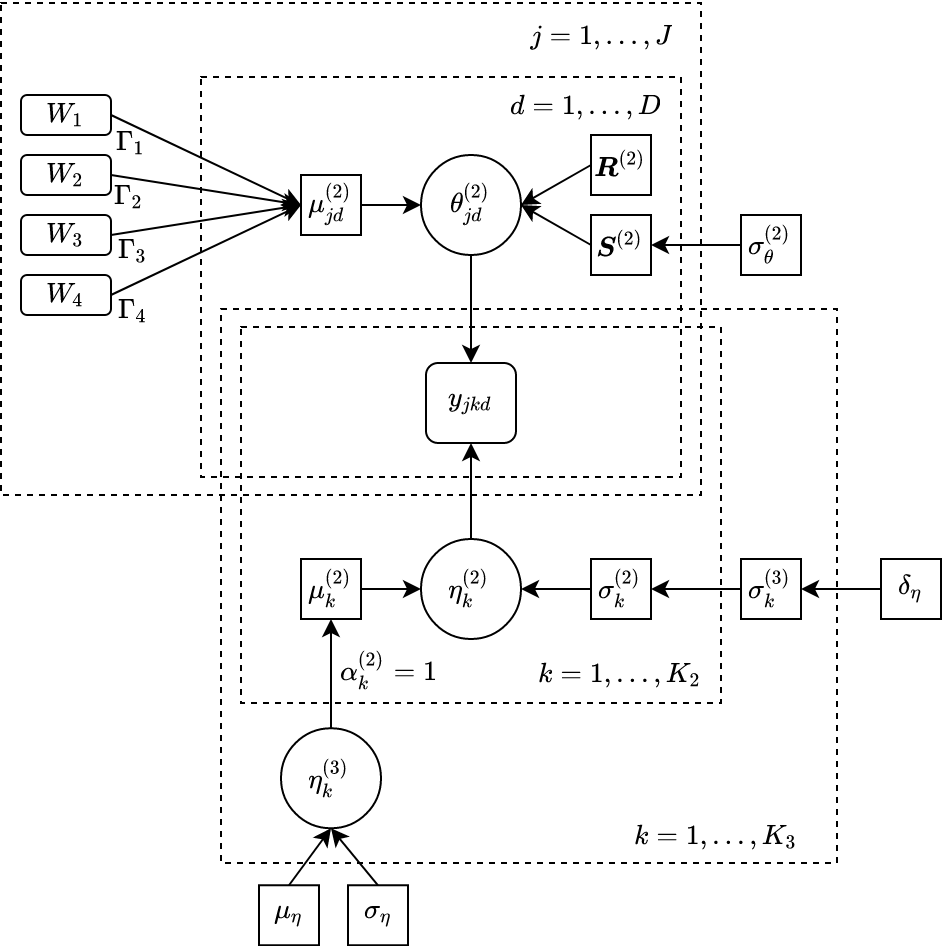
\includegraphics[width=0.7\linewidth]{4_FOLV_dag}
	%
	\caption[Directed Acyclig Graph (DAG). First Order Latent Variables model (FOLV).]%
	{Directed Acyclig Graph (DAG). First Order Latent Variables model (FOLV). Circles represent latent variables. Squares represent parameters or parameters for priors. Large Squares represent nesting in specific units.}
	\label{fig:FOLV_model}
\end{figure}
%
\begin{figure}[h]
	\centering
	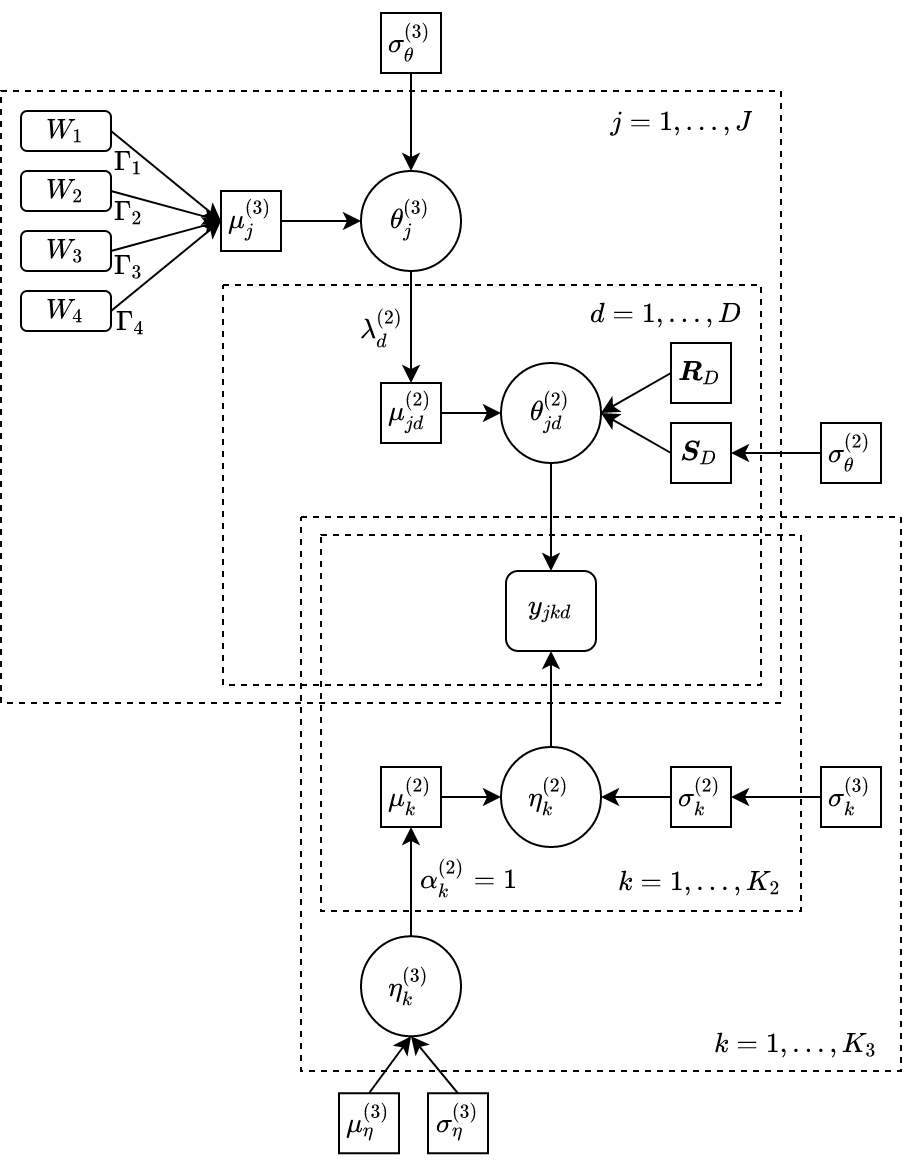
\includegraphics[width=0.8\linewidth]{4_SOLV_dag}
	%
	\caption[Directed Acyclic Graph (DAG). Second Order Latent Variables model (SOLV).]%
	{Directed Acyclig Graph (DAG). Second Order Latent Variables model (SOLV). Circles represent latent variables. Squares represent parameters or parameters for priors. Large Squares represent nesting in specific units.}
	\label{fig:SOLV_model}
\end{figure}

%%%%%%%%%%%%%%%%%%%%%%%%%%%%%%%%%%%%%%%%%%%%%%%%%%%%%%%%%%%%%%%%%%%%%%%

\section{Algorithm} \label{sect:algorithm}

Each data replication was simulated following a six-step procedure. First, the author randomly simulated a collection of pseudo-covariates $\mathbf{W}_{\theta} = [ W_{1}, W_{2}, W_{3}, W_{4} ]$, motivated by a similar information set present in the reading comprehension sub-test. The generated covariates were: (i) a binary ``gender" variable ($W_{1}$), describing males and females, (ii) an integer ``age" variable ($W_{2}$) with range $[30, 65]$, the latter corresponding to the age of retirement, (iii) a three-level categorical ``education" variable ($W_{3}$), indicating the type of education the individual received: institute only, university only, or both; and finally (iv) a four-level categorical ``experience" variable ($W_{4}$), denoting the individual's years of work experience, where the higher the category, the higher the years of experience. Associated with these, the author defined their regression parameters $\mathbf{\Gamma}_{\theta} = [\Gamma_{0}, \Gamma_{1}, \Gamma_{2}, \Gamma_{3}, \Gamma_{4}]$ where: (i) $\Gamma_{0} = 0$, indicating the absence of an intercept; (ii) $\Gamma_{1} = [\gamma_{m}, \gamma_{f}] = [0, 1]$, for males and females, respectively; (iii) $\Gamma_{2} = -0.01$, indicating the individuals loose ability with age, in a linear manner; (iv) $\Gamma_{3} = [\gamma_{io}, \gamma_{uo}, \gamma_{b}] = [-0.5, 0.5, 0]$, assuming individuals with only university degree have better ability levels, followed by individuals with both educations, and individuals with only institute degrees; and lastly (v) $\Gamma_{4} = [\gamma_{0y}, \gamma_{5y}, \gamma_{10y}, \gamma_{11+y}] = [-0.5, 0, 0.35, 0.5]$, implying experience has decreasing returns on abilities.

Second, the study simulated the second- and first-order latent variables, corresponding to the reading comprehension ability and its three sub-dimensions: literal, inferential and reflective. Reading comprehension ($\theta^{(3)}_{j}$) was generated from a normal distribution $N( \mu^{(3)}_{j}, \sigma^{(3)}_{\theta} )$, with $\mu^{(3)}_{j} = \pmb{\Gamma}_{\theta} \; \mathbf{W}_{\theta}$, i.e. the linear combination of the simulated covariates and its corresponding regression parameters, and $\sigma^{(3)}_{\theta}=0.5$. On the other hand, the three sub-dimensions were generated from a multivariate normal distribution $MVN( \pmb{\mu}^{(2)}_{j} , \pmb{\Sigma}^{(2)})$, with $\pmb{\mu}^{(2)}_{j} = [\mu^{(2)}_{j1}, \mu^{(2)}_{j2}, \mu^{(2)}_{j3}] = [\lambda^{(2)}_{1} \theta^{(3)}_{j}, \; \lambda^{(2)}_{2} \theta^{(3)}_{j}, \; \lambda^{(2)}_{3} \theta^{(3)}_{j} ]$, and $\pmb{\Sigma}^{(2)} = \mathbf{S}^{(2)} \cdot \mathbf{R}^{(2)} \cdot \mathbf{S}^{(2)}$. In order to ensure the FOLV model in figure \ref{fig:FOLV_model} lead us to the SOLV in figure \ref{fig:SOLV_model}, the author assumed loadings $\pmb{\lambda}^{(2)} = [\lambda^{(2)}_{1}, \lambda^{(2)}_{2}, \lambda^{(2)}_{3}] = [0.95, 0.95, 0.95]$. Using Wright's tracing rules \cite{Beaujean_2014}, the latter implies the sub-dimension would have an approximate unconditional correlation of $0.95 \times 0.94 = 0.9025$. Lastly, $\mathbf{S}^{(2)} = \pmb{\sigma}^{(2)}_{\theta} \mathbf{I}$, i.e. a diagonal standard deviation matrix with $\pmb{\sigma}^{(2)}_{\theta} = [0.5, 0.5, 0.5]$; whereas $\mathbf{R}^{(2)} = \mathbf{I}$, i.e. an identity correlation matrix, implying the sub-dimensions are independent after accounting reading comprehension.

Third, the author defined five ($5$) common stimulus or texts for the items, where the mean difficulty for the texts $\pmb{\eta}^{(3)} = [\eta^{(3)}_{1}, \eta^{(3)}_{2}, \eta^{(3)}_{3}, \eta^{(3)}_{4}, \eta^{(3)}_{5}] = [-1.50, -0.75, 0, 0.75, 1.50]$; whereas the deviation from said mean difficulties were $\sigma^{(3)}_{k} = 0.5$ for all texts. 

Fourth, $25$ items were randomly generated from independent normal distributions $N( \mu^{(2)}_{k}, \sigma^{(2)}_{k} ) $, with $\mu^{(2)}_{k} = \pmb{\eta}^{(3)} \pmb{\alpha}^{(2)} \mathbf{A}$ and $\sigma^{(2)}_{k} = \sigma^{(3)}_{k}$; where $\pmb{\alpha}^{(2)} = \mathbf{1}$, indicating the difficulty of the common stimulus directly explained the difficulty of the items, and $\mathbf{A}$ was a block design matrix that maps the items to its corresponding passage, defined in the previous step. Lastly, the dimensions the items were designed to measure were also generated at random.

Fifth, the author calculated the linear predictor $v_{jkd}$ and probability of endorsing an item $\pi_{jkd}$, for each individual $j$ on item $k$ (belonging to dimension $d$), according to equations (\ref{eq:linear_predictor2}), (\ref{eq:systematic}), and (\ref{eq:response_dich1}), respectively; where the probability was calculated using the logistic inverse-link function.
	
Sixth and last, the outcome $y_{jkd}$ was simulated from a Bernoulli distribution as in equation (\ref{eq:distributional}), with a probability of success calculated as in the previous step.

The code associated with the full simulation process can be found in Appendix \ref{appC2_1:sim}.

%%%%%%%%%%%%%%%%%%%%%%%%%%%%%%%%%%%%%%%%%%%%%%%%%%%%%%%%%%%%%%%%%%%%%%%
%%%%%%%%%%%%%%%%%%%%%%%%%%%%%%%%%%%%%%%%%%%%%%%%%%%%%%%%%%%%%%%%%%%%%%%

\section{Parameter estimation}

\subsection{Models and identification}

As stated in previous sections, we analyze two models: (i) the FOLV model depicted in figure \ref{fig:FOLV_model}, and (ii) the SOLV model depicted in figure \ref{fig:SOLV_model}. We proceed to enumerate the likelihood functions, and the full set of priors and hyper-priors used. 

First, as stated in equations (\ref{eq:dist}), (\ref{eq:lin_pred}) and (\ref{eq:prob}), the distributional and systematic part of both models was defined as follows:
%
\begin{align}
	%
	y_{jkd} &\sim \text{Bernoulli}( \pi_{jkd} ) \\
	%
	\text{logit}( \pi_{jkd} ) &= v_{jkd} \\
	%
	v_{jkd} &= \theta^{(2)}_{jd} - \eta^{(2)}_{k}
	%
\end{align}

Notice the linear predictor can be considered as a multilevel-multidimensional extension of the well known Rasch IRT model \cite{Rasch_1980}. As stated in previous chapters, the reader should keep in mind that in order to avoid the use of heavy notation, the items' indexes did not reflect the fact that some items are set to measure specific individual's dimensions. 

Second, the first-order latent variables and prior parameters were defined as follows:
%
\begin{align}
	%
	\boldsymbol{\theta}^{(2)}_{j} &= \left[ \theta_{j1}^{(2)}, \theta_{j2}^{(2)}, \theta_{j3}^{(2)} \right] \\
	%
	\boldsymbol{\theta}^{(2)}_{j} &\sim \text{MVNormal} \left( \boldsymbol{\mu}^{(2)}_{j}, \boldsymbol{\Sigma}^{(2)} \right)
	%
\end{align}

where $\boldsymbol{\Sigma}^{(2)}$ is defined by:
%
\begin{align}
	%
	\boldsymbol{\Sigma}^{(2)} &= \boldsymbol{S}^{(2)} \cdot \boldsymbol{R}^{(2)} \cdot \boldsymbol{S}^{(2)} \\
	%
	\boldsymbol{S}^{(2)} = \pmb{\sigma}^{(2)}_{\theta} \mathbf{I} &= 
	\begin{pmatrix}
		\sigma^{2}_{1}	& 0 			 	& 0 				\\
		0 				& \sigma^{2}_{2} 	& 0 				\\
		0 				& 0					& \sigma^{2}_{3} 
	\end{pmatrix} \\
	%
	\boldsymbol{R}^{(2)} &= 
	\begin{pmatrix}
		1			& \rho_{12} & \rho_{13} 	\\
		\rho_{21} 	& 1 		& \rho_{23} 	\\
		\rho_{31} 	& \rho_{32}	& 1	
	\end{pmatrix} 
	%
\end{align}

while $\boldsymbol{\mu}^{(2)}_{j}$ can be defined in two ways, depending on the model we are fitting. For the FOLV model depicted in figure \ref{fig:FOLV_model}, the mean vector would be defined as follows:
%
\begin{align}
	%
	\boldsymbol{\mu}^{(2)}_{j} &= \left[ \mu^{(2)}_{j1}, \; \mu^{(2)}_{j2}, \mu^{(2)}_{j3} \right] \\
	%
	\mu^{(2)}_{jd} &= \beta_{G} G_{j} + \beta_{A} (A_{j} - A_{\text{min}}) + \beta_{E} E_{j} + \beta_{X} X_{j}
	%
\end{align}

notice the regression parameters are not dimension specific. On the other hand, for the SOLV model depicted in figure \ref{fig:SOLV_model}, $\boldsymbol{\mu}^{(2)}_{j}$ would be defined by:
%
\begin{align}
	%
	\boldsymbol{\mu}^{(2)}_{j} &= \left[ \mu^{(2)}_{j1}, \; \mu^{(2)}_{j2}, \mu^{(2)}_{j3} \right] \\
	%
	\pmb{\lambda}^{(2)} &= \left[ \lambda^{(2)}_{1}, \; \lambda^{(2)}_{2}, \lambda^{(2)}_{3} \right] \\
	%
	\mu^{(2)}_{jd} &= \lambda^{(2)}_{d} \; \theta^{(3)}_{j} 
	%
\end{align}

where $d$ denotes the individual's dimension. Lastly, because the SOLV contemplates an additional level, corresponding to the reading comprehension ability, an additional set of parameters is defined as follows:
%
\begin{align}
	%
	\theta^{(3)}_{j} &\sim \text{Normal} \left( \mu^{(3)}_{j}, \sigma^{(3)}_{\theta} \right) \\
	%
	\mu^{(3)}_{j} &= \beta_{G} G_{j} + \beta_{A} (A_{j} - A_{\text{min}}) + \beta_{E} E_{j} + \beta_{X} X_{j}
\end{align}

Third, turning now our attention to the items' parameters $\eta^{(2)}_{k}$, for both models we have:
%
\begin{align}
	%
	\eta^{(2)}_{k} &\sim \text{Normal} \left( \mu^{(2)}_{k}, \sigma^{(2)}_{k} \right) \\
	%
	\mu^{(2)}_{k} &= \pmb{\eta}^{(3)} \mathbf{A} \\
	%
	\sigma^{(2)}_{k} &= \pmb{\sigma}^{(3)} \mathbf{A}
	%
\end{align}

where $k=1, \dots, 25$ items, $\pmb{\eta}^{(3)} = [ \eta^{(3)}_{1}, \eta^{(3)}_{2}, \eta^{(3)}_{3}, \eta^{(3)}_{4}, \eta^{(3)}_{5} ]$ represent the texts difficulties, $\pmb{\sigma}^{(3)} = [ \sigma^{(3)}_{1}, \sigma^{(3)}_{2}, \sigma^{(3)}_{3}, \sigma^{(3)}_{4}, \sigma^{(3)}_{5} ]$ the text deviations from such difficulties; and $\mathbf{A}$ is the block matrix that maps the items with its corresponding passage. In addition, $\eta^{(3)}_{k}$ and $\sigma^{(3)}_{k}$ are distributed as:
%
\begin{align}
	%
	\eta^{(3)}_{k} &\sim \text{Normal} \left( \mu_{\eta}, \sigma_{\eta} \right) \\
	%
	\sigma^{(3)}_{k} &\sim \text{Exponential} \left( \delta_{\eta} \right)
	%
\end{align}

Fourth, we declared all the hyper-priors required:
%
\begin{align}
	\boldsymbol{R}^{(2)} &\sim \text{LkjCorrelation}( 2 ) \\
	\beta_{G} &\sim \text{Normal}( 0, 0.5 ) \\
	\beta_{A} &\sim \text{Normal}( 0, 0.5 ) \\
	\beta_{E} &\sim \text{Normal}( 0, 1 ) \\
	\beta_{X} &\sim \text{Normal}( 0, 0.5 ) 
	%
\end{align}

\noindent where $\text{LkjCorrelation}(\cdot)$ denotes the Lewandowski, Kurowicka, and Joe correlation distribution \cite{Lewandowski_et_al_2009}. 

Finally, in order to fully specify the model and provide a scale for the latent variables, the current research decided to set the scale of the higher order dimension and sub-dimensions to one, i.e. $\sigma^{(3)}_{\theta} = 1$, and $\mathbf{S}^{(2)} = \pmb{\sigma}^{(2)}_{\theta} \mathbf{I}$ with $\pmb{\sigma}^{(2)}_{\theta} = [1, 1, 1]^{T}$, commonly know as the unit variance identification scheme (UVI). Moreover, to identify the texts' and items' parameters we set $\mu_{\eta} = 0$, $\sigma_{\eta}=1$, $\delta_{\eta}=2$.

Notice we need to set the scales for all the dimensions equal to one, because otherwise the latent structure would not be identified. At the level of the FOLV (level-2), we would have $(3 \times 4)/2 = 6$ pieces of information available, corresponding to the variances and covariances of the FOLV. The information then will need to estimate $10$ parameters, i.e. $3$ loadings, $4$ variances corresponding to the FOLV and SOLV, and $3$ correlations among sub-dimensions. Therefore, by restricting the variances to one, we have enough information to estimate the other parameters of interest (loadings and correlations). Additionally, this is further justified by the fact that latent variables have no inherent unit in which they are measured, consequently, setting their scale is an arbitrary  decision \cite{Beaujean_2014}.


\begin{comment}
On the other hand, from the texts and items perspective, at the level of the items (level-2) we would have $(25 \times 26)/2 = 325$ pieces of information available, corresponding to the variances and covariances of the items dimensions. With that information we would need to estimate $30$ parameters, corresponding to $25$ items' dimension variances, and $5$ texts' dimension variances. notice in this case, we do not need to estimate $25$ loadings, as they are assumed to be $1$.
\end{comment}

%%%%%%%%%%%%%%%%%%%%%%%%%%%%%%%%%%%%%%%%%%%%%%%%%%%%%%%%%%%%%%%%%%%%%%%

\subsection{Prior predictive investigation}

As it was outlined in section \ref{sub_sect:prior_pred}, we will use prior predictive investigation to assess and visualize the consequences of our prior assumptions. The implications will be assessed from two perspectives: the IRT and the outcome space perspective. For the former, we will investigate what the set of priors imply for the item characteristic curves (ICC), and item information function (IIF). For the latter, we will examine how the prior assumption translate onto the outcome space.

First, it will useful to define the ICC and IIF functions. \citet{Hambleton_et_al_1991b} defined the ICC as the mathematical function that relates the probability of success on an item, to the ability measured by that same item. In our current implementation, such function would correspond to the systematic part of the GLLAMM, as defined in equations (\ref{eq:systematic}) and (\ref{eq:response_dich1}):
%
\begin{equation} \label{eq:ICC}
	\begin{split}
		\text{ICC} &= \pi_{jkd} = \frac{ \text{exp}(v_{jkd}) }{ 1 + \text{exp}(v_{jkd}) }
	\end{split}	
\end{equation}

\noindent where the linear predictor $v_{jkd}$ contains the items' dimensions $\eta^{(m)}_{k}$ and the individuals' abilities $\theta^{(l)}_{jd}$, as defined in equation \ref{eq:linear_predictor1}. As previously mentioned, the ICC of our current implementation can be considered as the multilevel-multidimensional extension to the Rasch model's ICC.

On the other hand, the same authors defined the IIF as a function that measured the amount of information provided by an item. In this setting, ``information" is understood as the reduction of uncertainty, resulting from using an item to measure the ability of an individual. Given the above, the IIF for the GLLAMM will be defined as in its Rasch counterpart, in the following form:
%
\begin{equation} \label{eq:IIF}
	\begin{split}
		\text{IIF} &= \pi_{jkd} \; (1 - \pi_{jkd})
	\end{split}	
\end{equation}

Figure \ref{fig:FOLV_ICC_prior} shows the ICC and IIF for the FOLV (figure \ref{fig:FOLV_model}), resulting from the assumptions integrated by the priors detailed in the previous section. From panel (A), we can notice the difficulty of the items match a wide range of the individuals' abilities (see multiple black solid lines). This means that the model expect items' difficulties to be in any part of the continuous range of abilities, with no restriction. Furthermore, the latter imply the priors allow the model to obtain information about individuals, located in the full significant range of the abilities, as seen in panel (B) of the same figure. All of this just means that no unintended assumption has ``creep" into the model, at least from the IRT perspective. A similar result can be seen for the SOLV (figure \ref{fig:SOLV_ICC_prior}, appendix).
%
\begin{figure}[H]
	\centering
	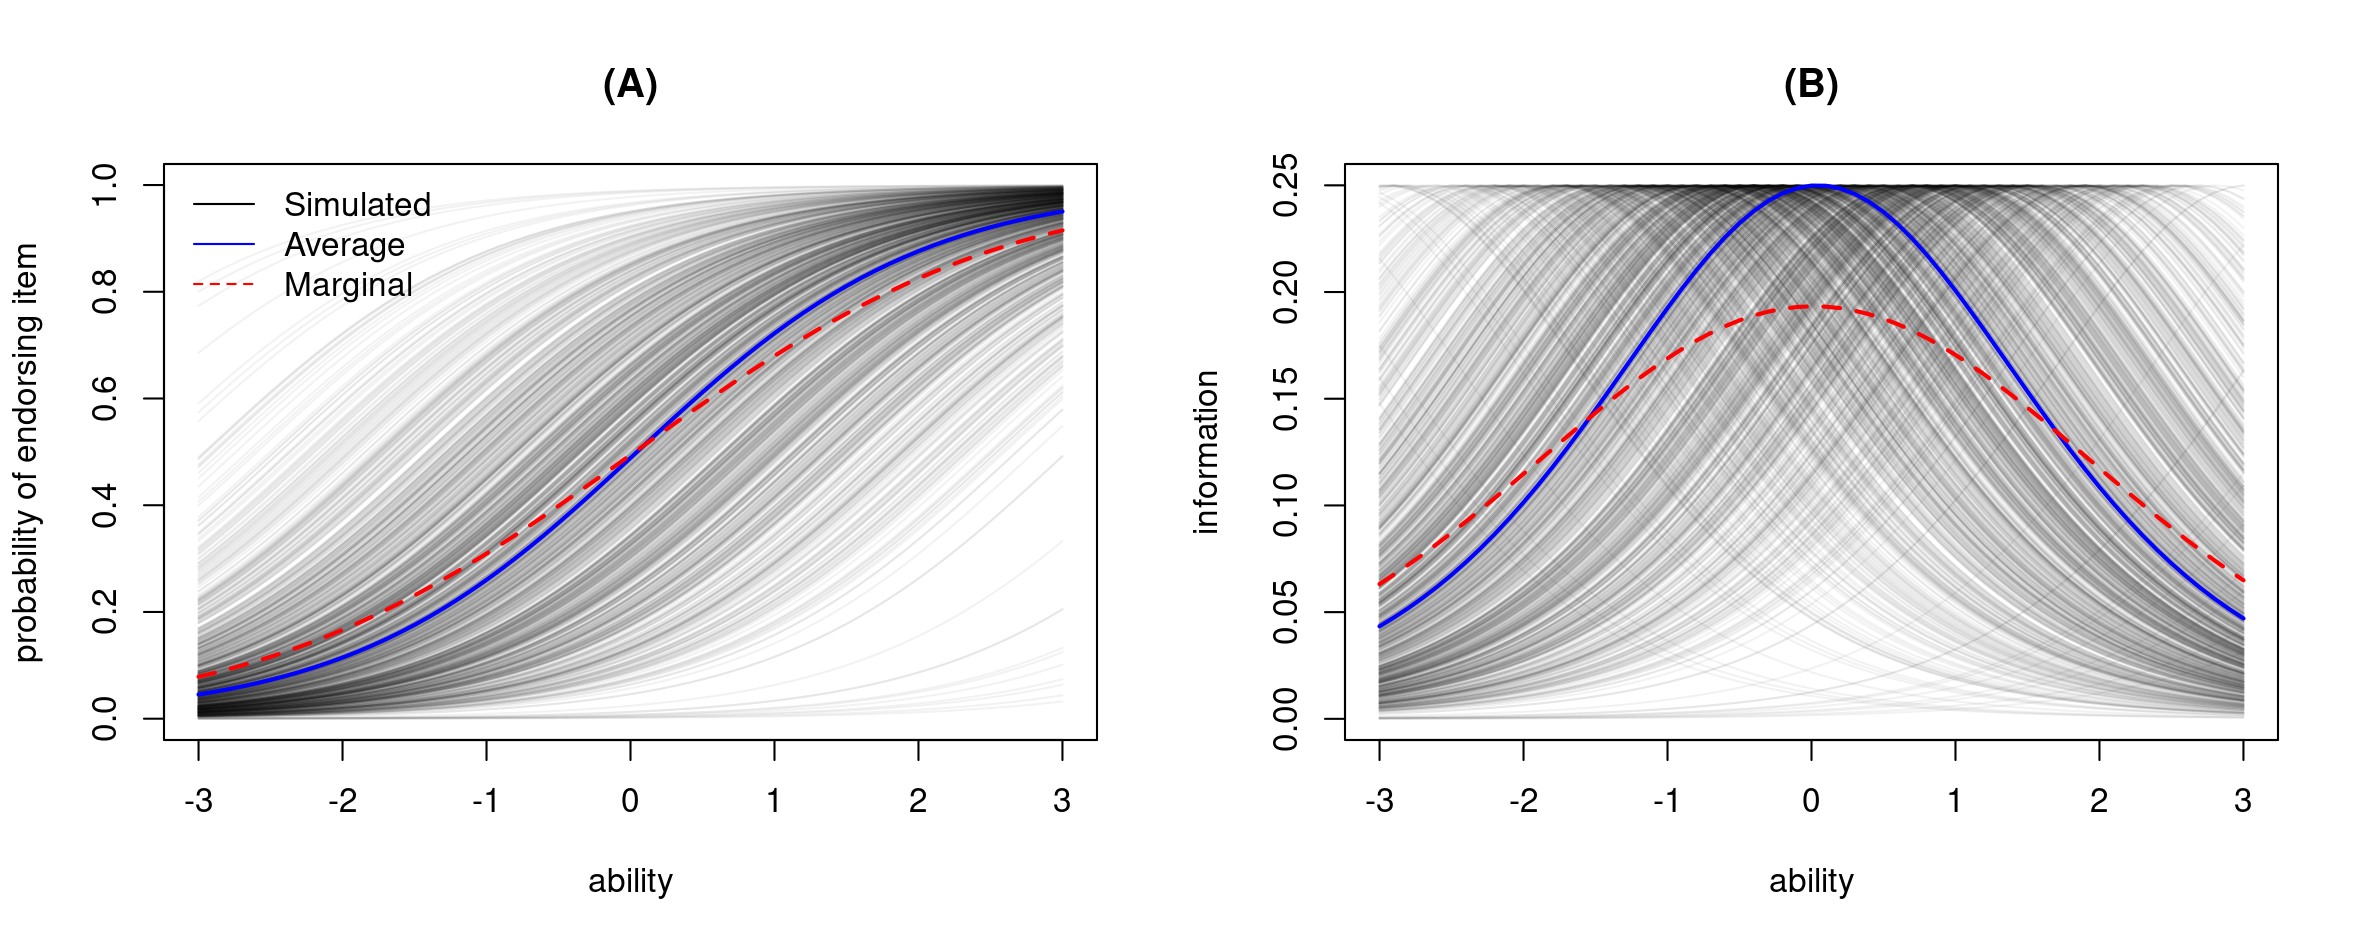
\includegraphics[width=1\linewidth]{FOLV_ICC_prior}
	%
	\caption[First-Order latent variable model (FOLV). Item Characteristic Curve (ICC) and Item Information Function (IIF).]%
	{First-Order latent variable model (FOLV). (A) Item Characteristics Curve, ICC. (B) Item Information Function, IIF.}
	\label{fig:FOLV_ICC_prior}
\end{figure}

Finally, from figure \ref{fig:FOLV_hitrate1} and \ref{fig:FOLV_hitrate2}, we notice that no unintended assumption has been translated to the outcome space of the FOLV either. Panel (A) from figure \ref{fig:FOLV_hitrate1} shows the individuals'  proportion of correctly answered items, can be present in the full range of possibilities. Furthermore, panel (B) of the same figure, shows the proportion of individuals endorsing an item, for any item, can also be present in the full range of possibilities. Lastly, panels (C) and (D) convey similar information aggregated by texts and dimensions. On the other hand, from all panels in figure \ref{fig:FOLV_hitrate2}, we can observe the priors did not force the model to assume any apriori tendency in the covariates. A similar result can be seen for the outcome space of the SOLV (figures \ref{fig:SOLV_hitrate1} and \ref{fig:SOLV_hitrate2}, appendix).
%
\begin{figure}[h]
	\centering
	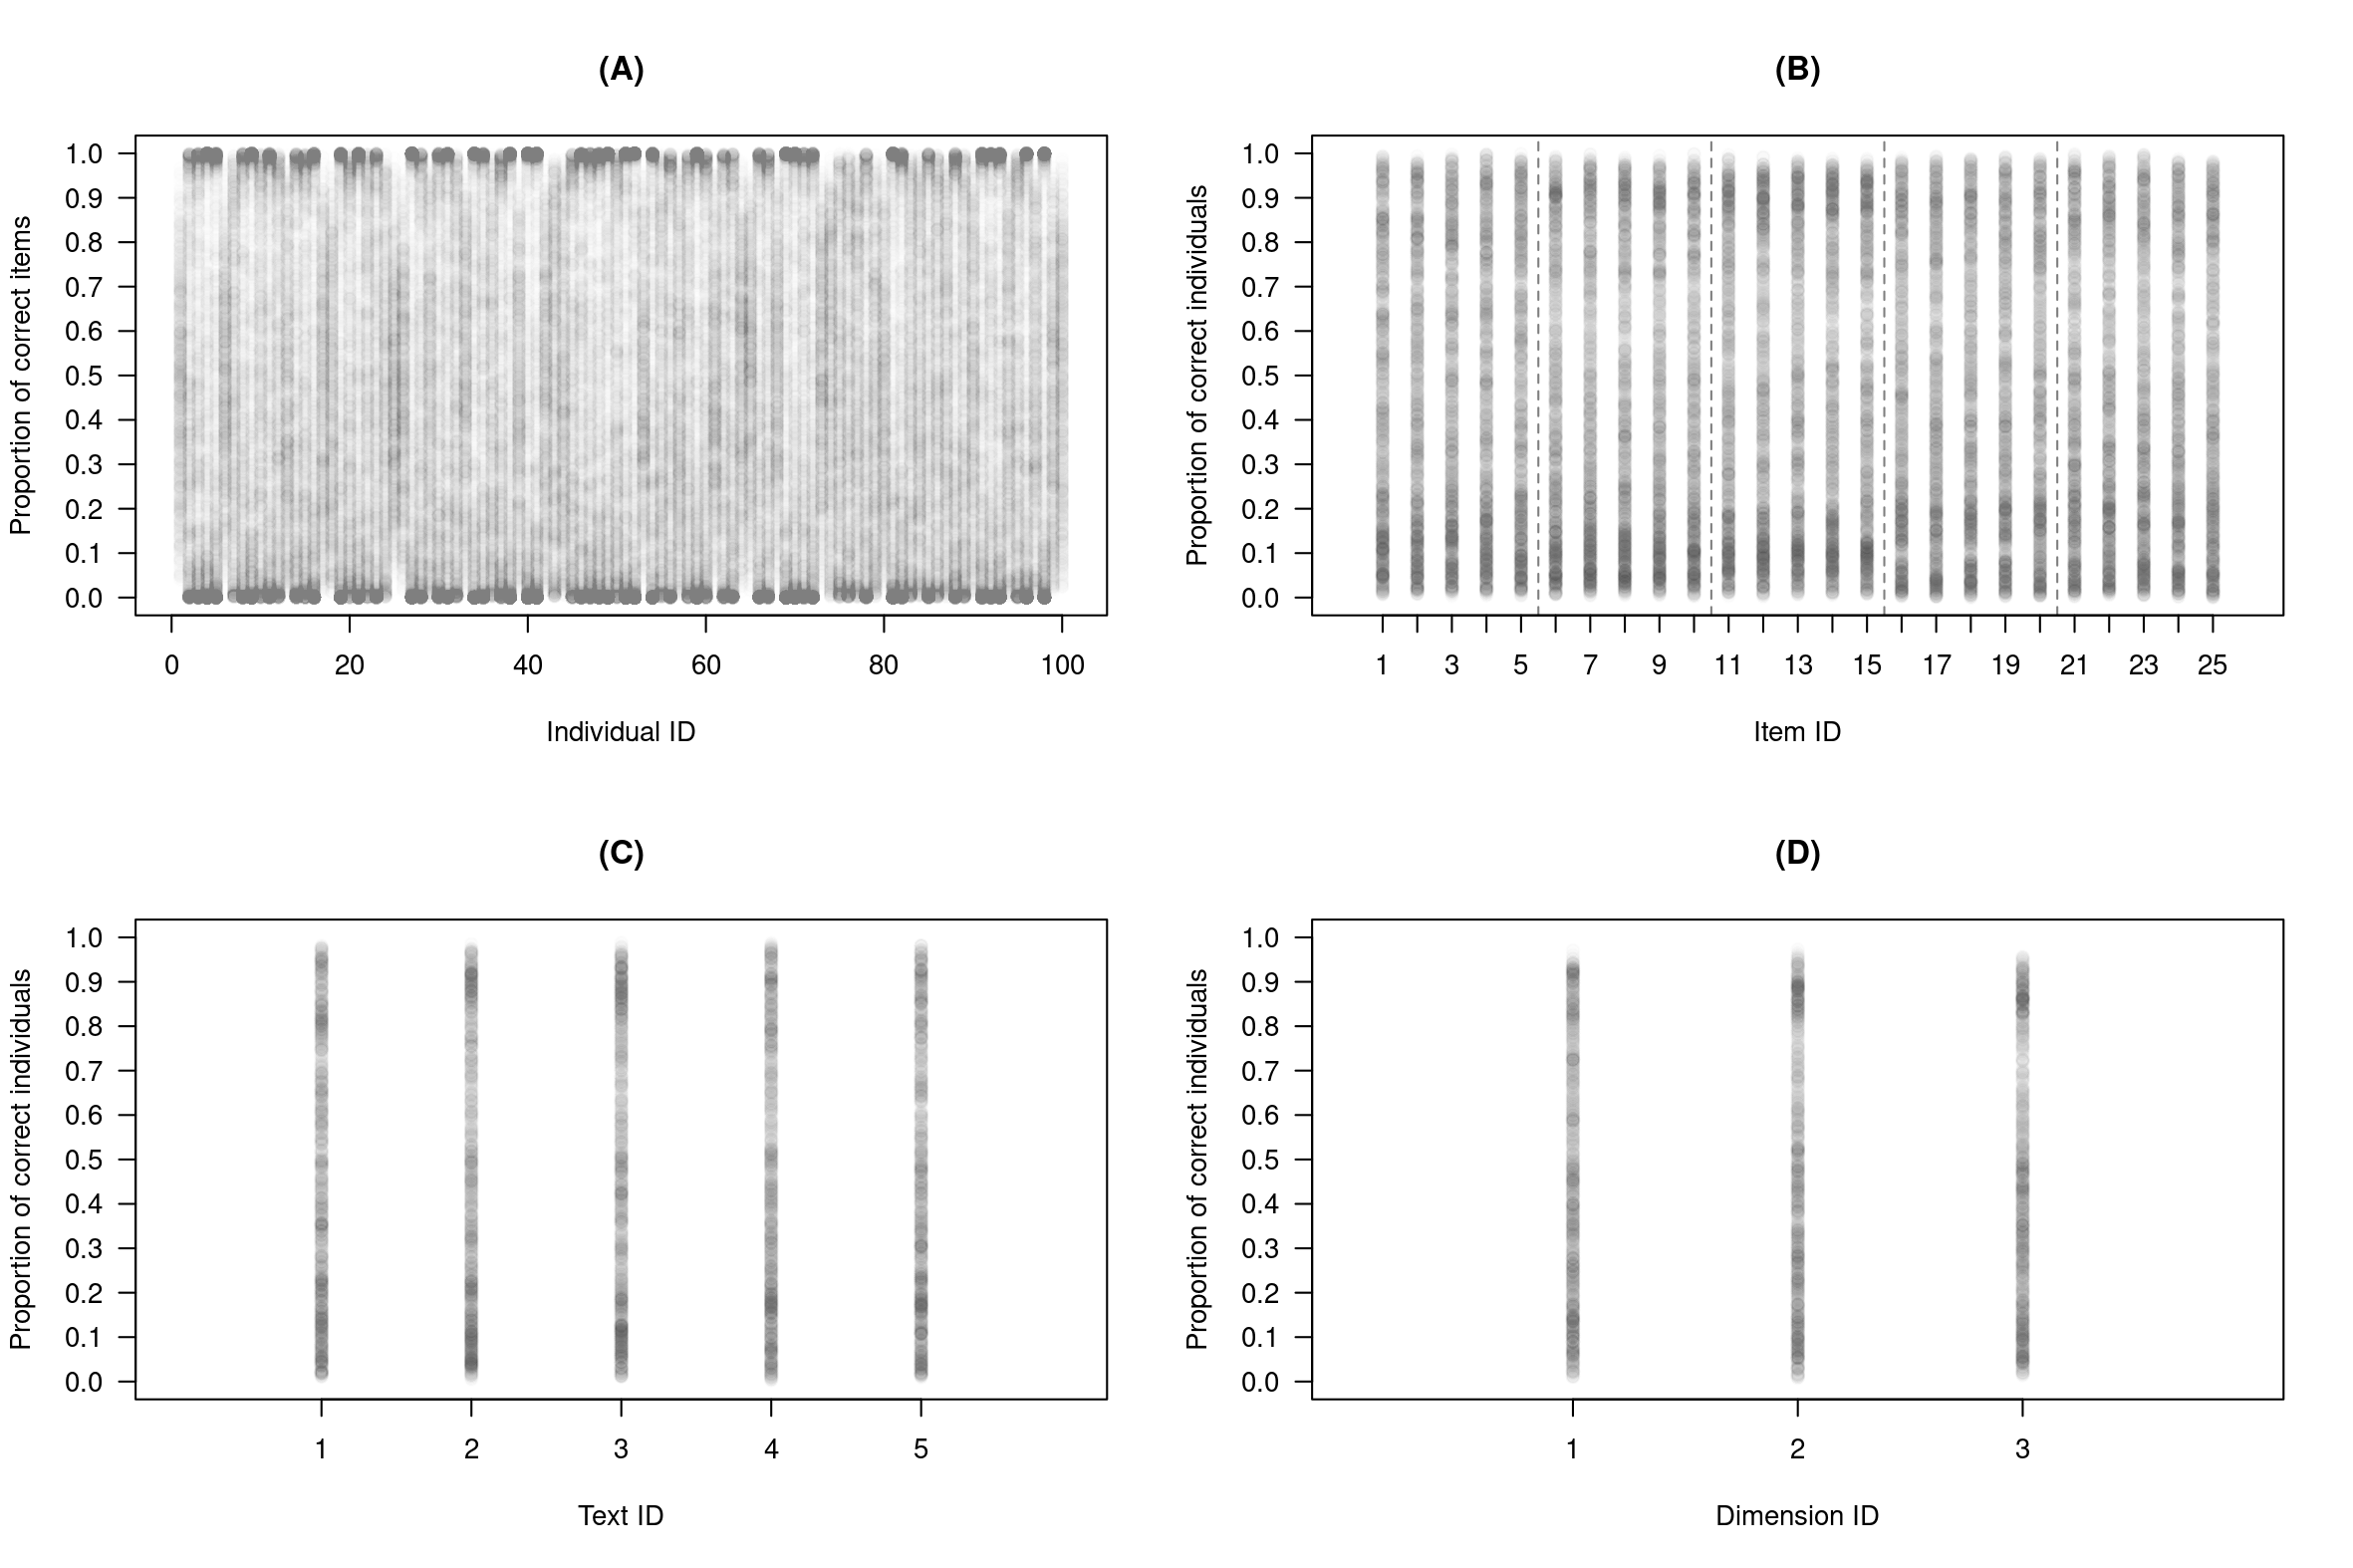
\includegraphics[width=1\linewidth]{FOLV_HitRate1}
	%
	\caption[First-Order latent variable model (FOLV). Hit rate per dimensions of interest.]%
	{First-Order latent variable model (FOLV). Aggregated endorsement rate per: (A) individuals, (B) items, (C) text or passage, and (D) measured dimension.}
	\label{fig:FOLV_hitrate1}
\end{figure}
%
\begin{figure}[h]
	\centering
	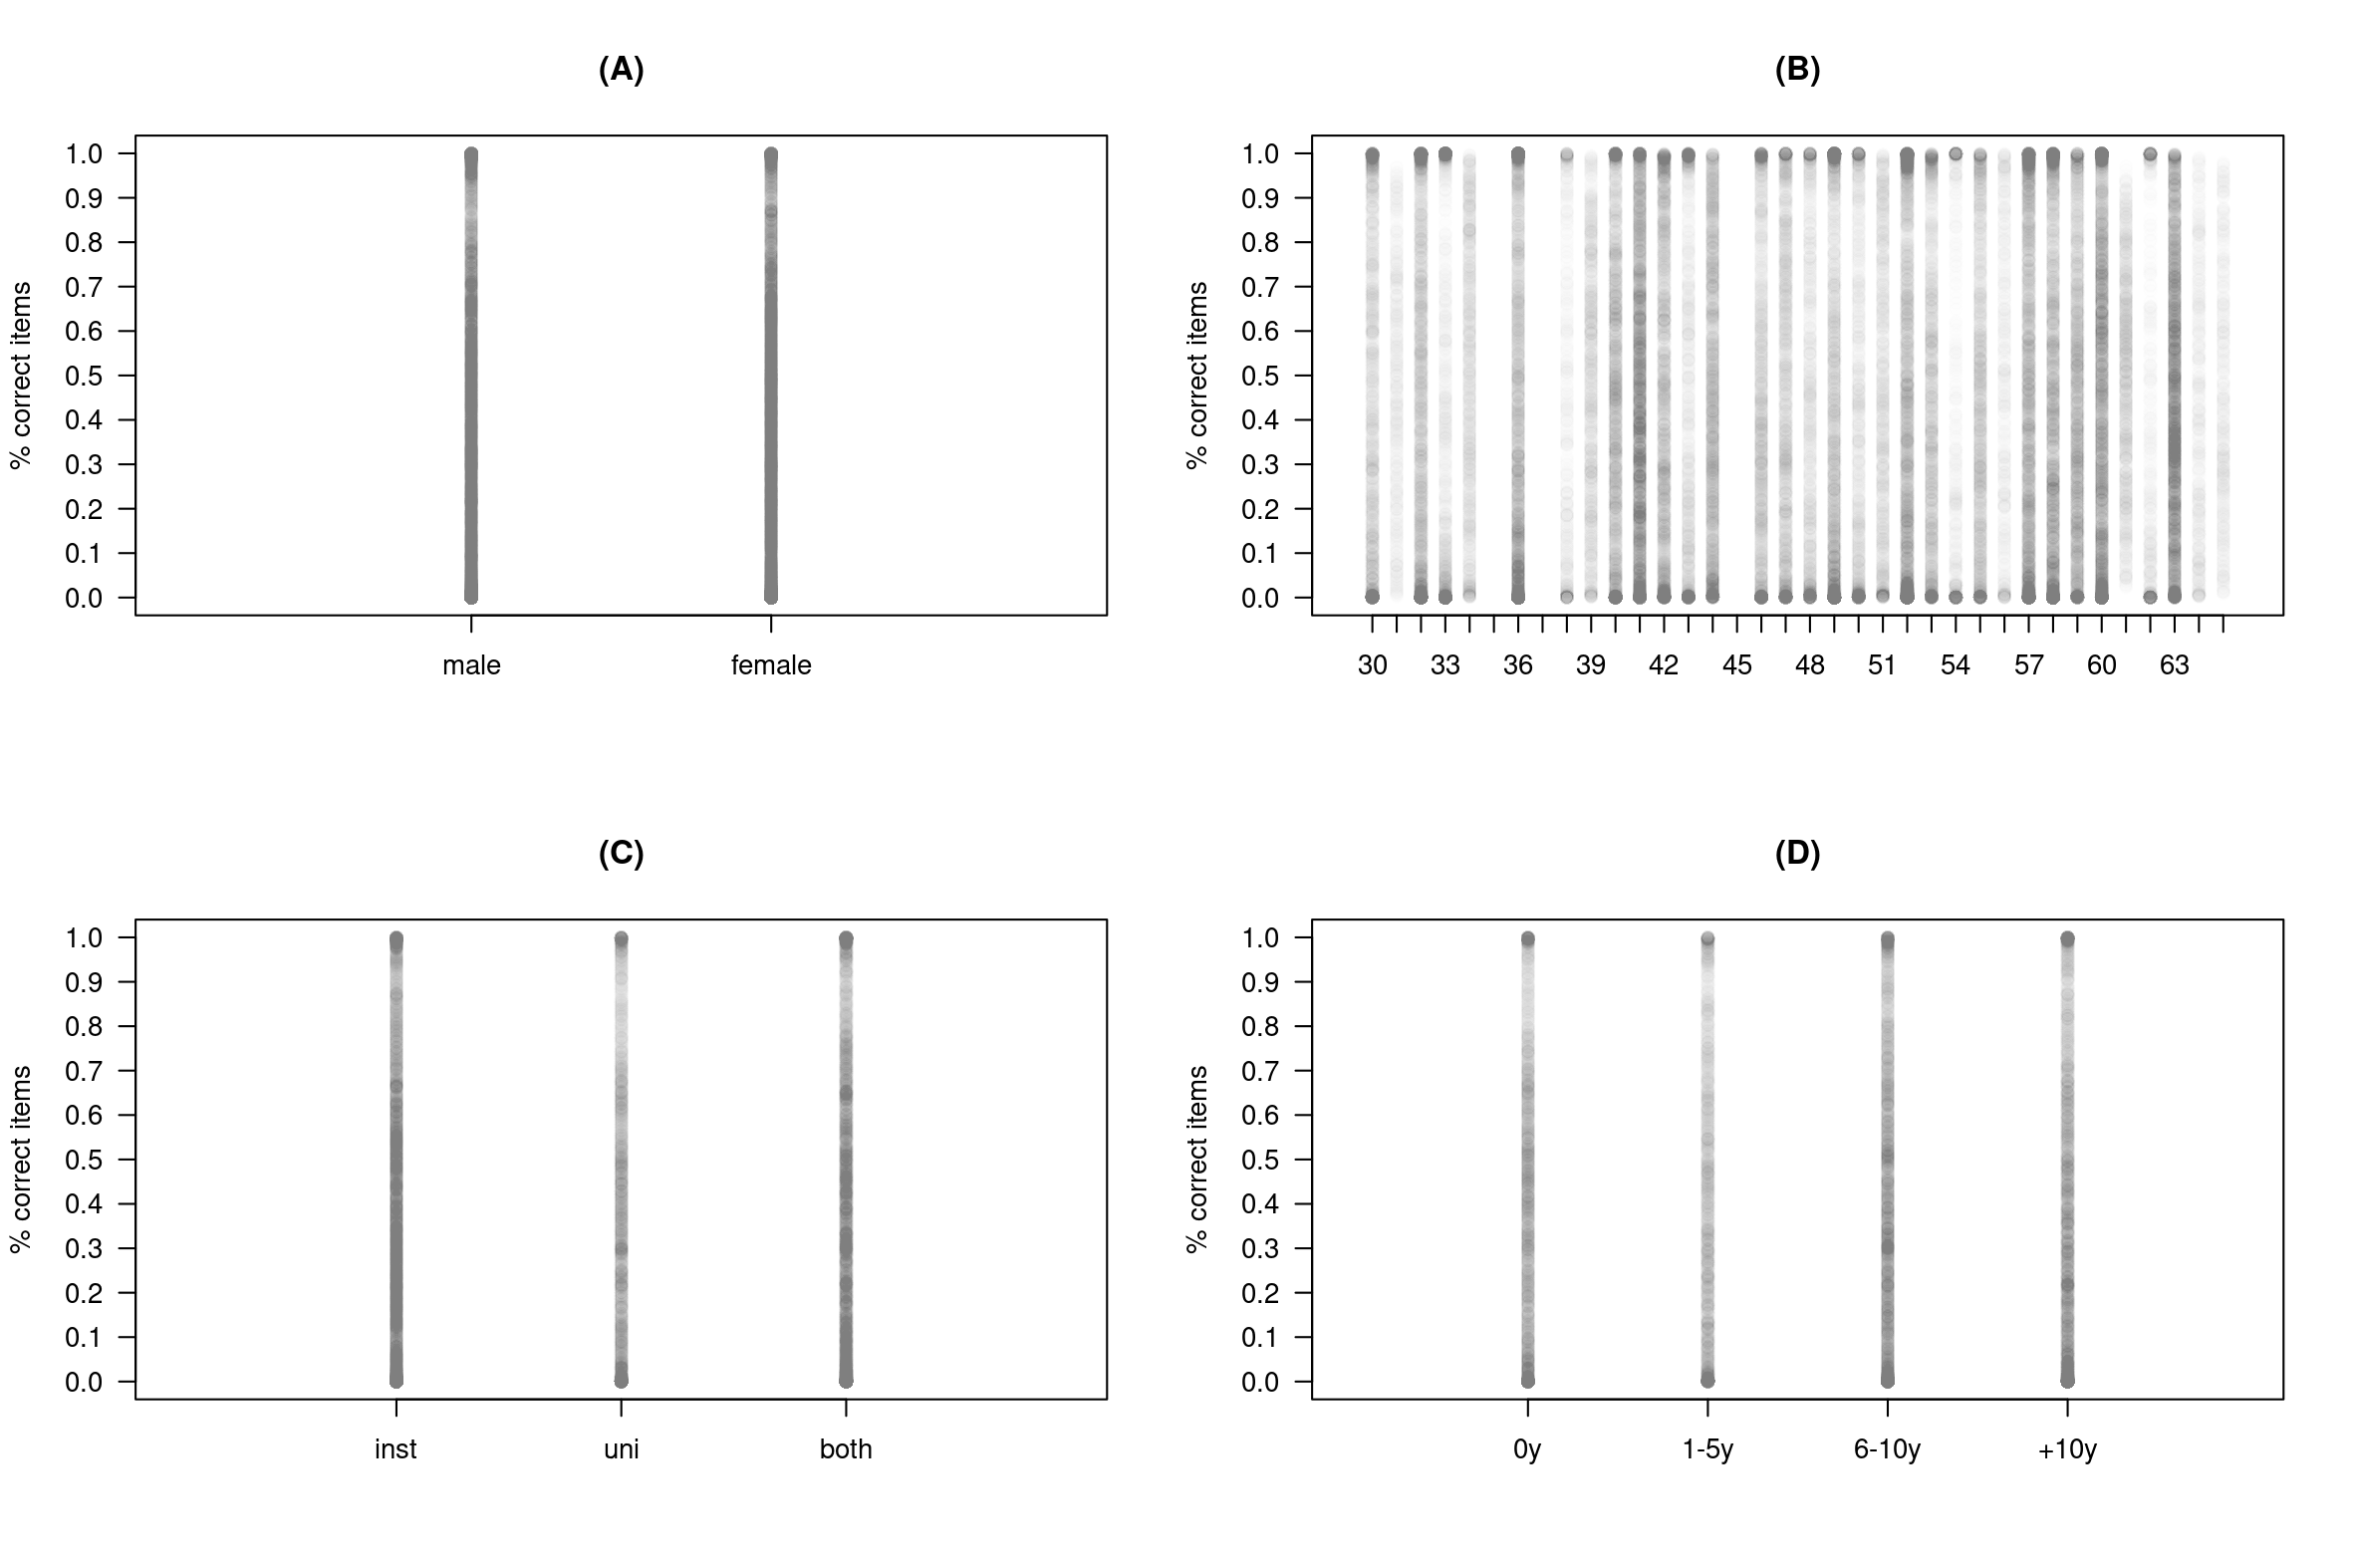
\includegraphics[width=1\linewidth]{FOLV_HitRate2}
	%
	\caption[First-Order latent variable model (FOLV). Hit rate per simulated covariate.]%
	{First-Order latent variable model (FOLV). Aggregated endorsement rate per simulated covariate: (A) gender, (B) age, (C) education, and (D) experience.}
	\label{fig:FOLV_hitrate2}
\end{figure}

%%%%%%%%%%%%%%%%%%%%%%%%%%%%%%%%%%%%%%%%%%%%%%%%%%%%%%%%%%%%%%%%%%%%%%%
%%%%%%%%%%%%%%%%%%%%%%%%%%%%%%%%%%%%%%%%%%%%%%%%%%%%%%%%%%%%%%%%%%%%%%%

\section{Evaluation criteria}

As stated in section \ref{sec:conditions}, the study was set to evaluate the performance, recovery capacity, and retrodictive accuracy of the bayesian implementation.

First, to assess the performance of the MCMC chains, in terms of achieving stationarity, convergence and good mixing, the author followed the usual visual approach. The approach involved the visual evaluation of (i) trace plots, for stationarity and convergence, and (ii) trank and autocorrelation plots (ACF), for good mixing. Moreover, the assessment of convergence and good mixing were supported by the \texttt{Rhat} and \texttt{n\_eff} statistics developed in \citet{Gelman_et_al_2014} (pp. $284-287$).

Second, to evaluate the recovery capacity for all parameters $\pmb{\Omega} = \{ \pmb{\beta}, \pmb{\Lambda}, \pmb{\Theta}, \pmb{\Psi}, \pmb{\Gamma} \}$, the author used the root mean squared error (RMSE), i.e. the extent of the deviation the posterior means exhibited from the true generating values, in all replicate simulations. Notice, in the case of the FOLV model no loading recovery can be assessed; however, using Wright's tracing rules, we evaluated the implied correlation structure between the sub-dimensions, resulting from having a second-order latent variable. The RMSE for each parameter of interest was defined as follows:
%
\begin{align}
	%
	RMSE \left( \eta^{(m)}_{k} \right) &=\sqrt{\frac{1}{R} \sum_{r=1}^{R} \left( \hat{\eta}^{(m)}_{kr} - \eta^{(m)}_{k} \right)^2}
	%
\end{align}
%
\begin{align}
	%
	RMSE \left( \theta^{(l)}_{jd} \right) &=\sqrt{\frac{1}{R} \sum_{r=1}^{R} \left( \hat{\theta}^{(l)}_{jdr} - \theta^{(l)}_{jd} \right)^2} \\
	%
	RMSE \left( \Gamma_{w} \right) &=\sqrt{\frac{1}{R} \sum_{r=1}^{R} \left( \hat{\Gamma}_{wr} - \Gamma_{w} \right)^2} \\
	%
	%
	RMSE \left( \lambda^{(l)}_{d} \right) &=\sqrt{\frac{1}{R} \sum_{r=1}^{R} \left( \hat{\lambda}^{(l)}_{dr} - \lambda^{(l)}_{d} \right)^2}
	%
\end{align}

\noindent where the ``hat" parameters with index $r$ described the posterior mean in replica $r=1, \dots, R$, with $R=10$, and each posterior mean was calculated with $3$ chains of $1,000$ iterations each.

Finally, since IRT models are known to be invariant to the shift of the linear predictor \cite{Baker_et_al_1992, Bock_1972}, i.e. the addition/subtraction of a constant to the abilities/difficulties results in the same probability value, it could happen that we observe substantial differences in the recovery of the parameters, that not necessarily implies a classification error  \cite{Wollack_2002}. Therefore, to avoid a mistake in the assessment of fit of the model, the current research will use posterior predictive checks, i.e. retrodictive accuracy. 

{ \color{red} What are they?, at which aggregattion dimensions?: for individuals in different dimensions, items, and texts. }



%%%%%%%%%%%%%%%%%%%%%%%%%%%%%%%%%%%%%%%%%%%%%%%%%%%%%%%%%%%%%%%%%%%%%%%
%%%%%%%%%%%%%%%%%%%%%%%%%%%%%%%%%%%%%%%%%%%%%%%%%%%%%%%%%%%%%%%%%%%%%%%

\section{Results}

\subsection{Chain performance}

First, the CP and NCP chain performance for the texts' mean difficulties is reported in figures \ref{fig:FOLV_CE_chains1} and \ref{fig:FOLV_NC_chains1}, respectively. The figures correspond to replica number two of the FOLV model, with a simulated sample size of $100$. 

From the figures, one can easily notice the parameters under the CP did not show signs of achieving ergodicity. The chains showed a clear lack of stationarity and convergence (left panels). Moreover, the iterations did not explore the posterior distribution appropriately, hinting a lack of good mixing, e.g. the top trace and trank plots show chains that are ``stuck" in specific areas of the distribution. In addition, the ACF plots reveal the chain iterations were highly auto-correlated, again indicating a serious lack of good mixing. All of this is further confirmed by panels (A) and (C) of figure \ref{fig:FOLV_stat1}, where we can see the CP has low effective samples sizes (\texttt{n\_eff}) and higher than appropriate \texttt{Rhat} values, compared to the NCP.

On the contrary, the parameters from the NCP seem to achieve ergodicity. The trace plots show chains that seem to be stationary and convergent. The trank plots show the rapid exploration of the full range of posterior distribution. And finally, the ACF plots show the iterations were less auto-correlated. Again, this is further confirmed by figure \ref{fig:FOLV_stat1}, where the NCP show greater \texttt{n\_eff} and appropriate \texttt{Rhat} values, versus the CP.

On the other hand, figures \ref{fig:FOLV_CE_chains2} and \ref{fig:FOLV_NC_chains2} (appendix) show the the CP and NCP trace, trank, and ACF plots for the the difficulties' deviations of the texts. At a simple glance, the plots seem to indicate that both parametrizations achieve a similar level of ergodicity. However, from panels (A) and (C) in figure \ref{fig:FOLV_stat1}, we can notice that while both parametrization show an \texttt{Rhat}$<1.05$, the CP effectively has sample sizes in a larger range than the NCP, i.e. $[35, 2734]$ and $[897, 2587]$, respectively. The latter just indicates the NCP has less auto-correlated chains, and therefore a bit better mixing.

Furthermore, figures \ref{fig:FOLV_CE_chains3} and \ref{fig:FOLV_NC_chains3} (appendix) show the chain performance for the item difficulties under the CP and NCP, respectively. The trace, trank and ACF plots show a similar pattern as the one outlined for the difficulty of the texts, albeit more extreme. The CP chains did not achieved stationarity, convergence, nor good mixing; whereas it seems the NCP does. This is further confirmed by panels (B) and (D) of figure \ref{fig:FOLV_stat1}, where one can see the NCP has significantly higher effective sample sizes and \texttt{Rhat}$<1.05$, in contrast to the CP.

Second, the chain performance for the reading comprehension sub-dimensions, under the CP are reported in figures \ref{fig:FOLV_CE_chains4}, \ref{fig:FOLV_CE_chains5}, \ref{fig:FOLV_CE_chains6}. The figures correspond to replica number six of the FOLV model, with a simulated sample size of $100$. The chains also show a lack of ergodicity similar to the texts' difficulties, e.g. the left panels of figure \ref{fig:FOLV_CE_chains6} show chains that did not explore the posterior distribution appropriately (see straight lines in chains). This is further confirmed by panels (A) through (D) in figure \ref{fig:FOLV_stat3}, where the CP has effective sample sizes in the range of $[8, 527]$, while an important proportion of the parameters is above the recommended \texttt{Rhat} threshold. In contrast, the NCP chains for the sub-dimensions achieve ergodicity, as it is shown in figures \ref{fig:FOLV_NC_chains4}, \ref{fig:FOLV_NC_chains5}, \ref{fig:FOLV_NC_chains6} and confirmed by the \texttt{n\_eff} and \texttt{Rhat} values in figure \ref{fig:FOLV_stat3}.

Third, similar visualizations for the CP and NCP regression parameters are shown in figures \ref{fig:FOLV_CE_chains7} and \ref{fig:FOLV_NC_chains7}. With a careful inspection of the CP trace plots, one can notice we still have chains that are ``stuck" in specific part of the posterior distribution (see green lines). As a result, the CP registered lower effective samples sizes than the NCP, as figure \ref{fig:FOLV_stat2} confirms. However, neither of those things prevented the CP achieving convergence, as the \texttt{Rhat} in the same figure confirms. In contrast, the NCP parameters seem to achieve stationarity, convergence, and good mixing without any issues, with higher effective sample sizes and \texttt{Rhat} values close to one.
%
\begin{figure}[H]
	\centering
	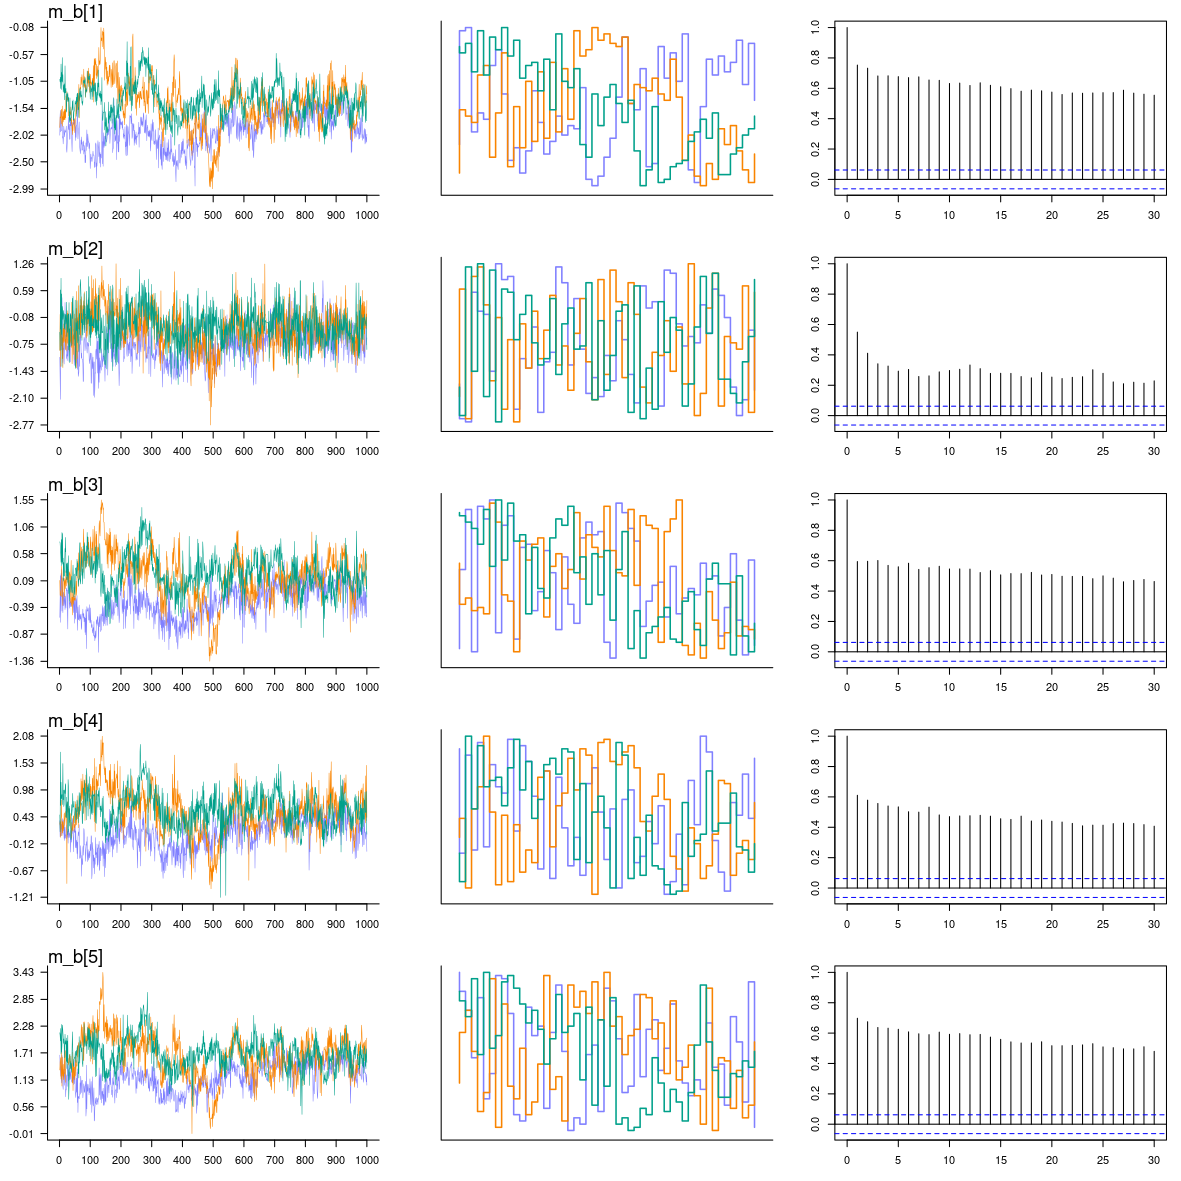
\includegraphics[width=1\linewidth]{FOLV_CE_J100_Ndata2_mb}
	%
	\caption[First-Order latent variable model (FOLV). Sample size $100$, replica number $2$. Centered parametrization. Mean difficulty per text. Trace, trank and auto-correlation plots.]%
	{First-Order latent variable model (FOLV). Sample size $100$, replica number $2$. Centered parametrization. Mean difficulty per text: (Left) trace plot, (Middle) trank plot, (Right) auto-correlation plot.}
	\label{fig:FOLV_CE_chains1}
\end{figure}

Lastly, the performance assessment plots for the FOLV sub-dimensions' correlation are shown in figures \ref{fig:FOLV_CE_chains8} and \ref{fig:FOLV_NC_chains8}. In both parametrizations, we observe the correlations seem to achieve stationarity and convergence. However, it also seems they do not achieve good mixing, i.e. the MCMC procedure does not manage to make a proper investigation of the posterior. This is further confirmed by panels (B) and (D) from figure \ref{fig:FOLV_stat2}, where we see observe the parameters' chains remain below the \texttt{Rhat} recommended threshold, indicating convergence. Although, the effective sample sizes were low, in the range of $[249, 1311]$ for CP, and $[285, 1283]$ for NCP, indicating highly auto-correlated iterations. 
%
\begin{figure}[H]
	\centering
	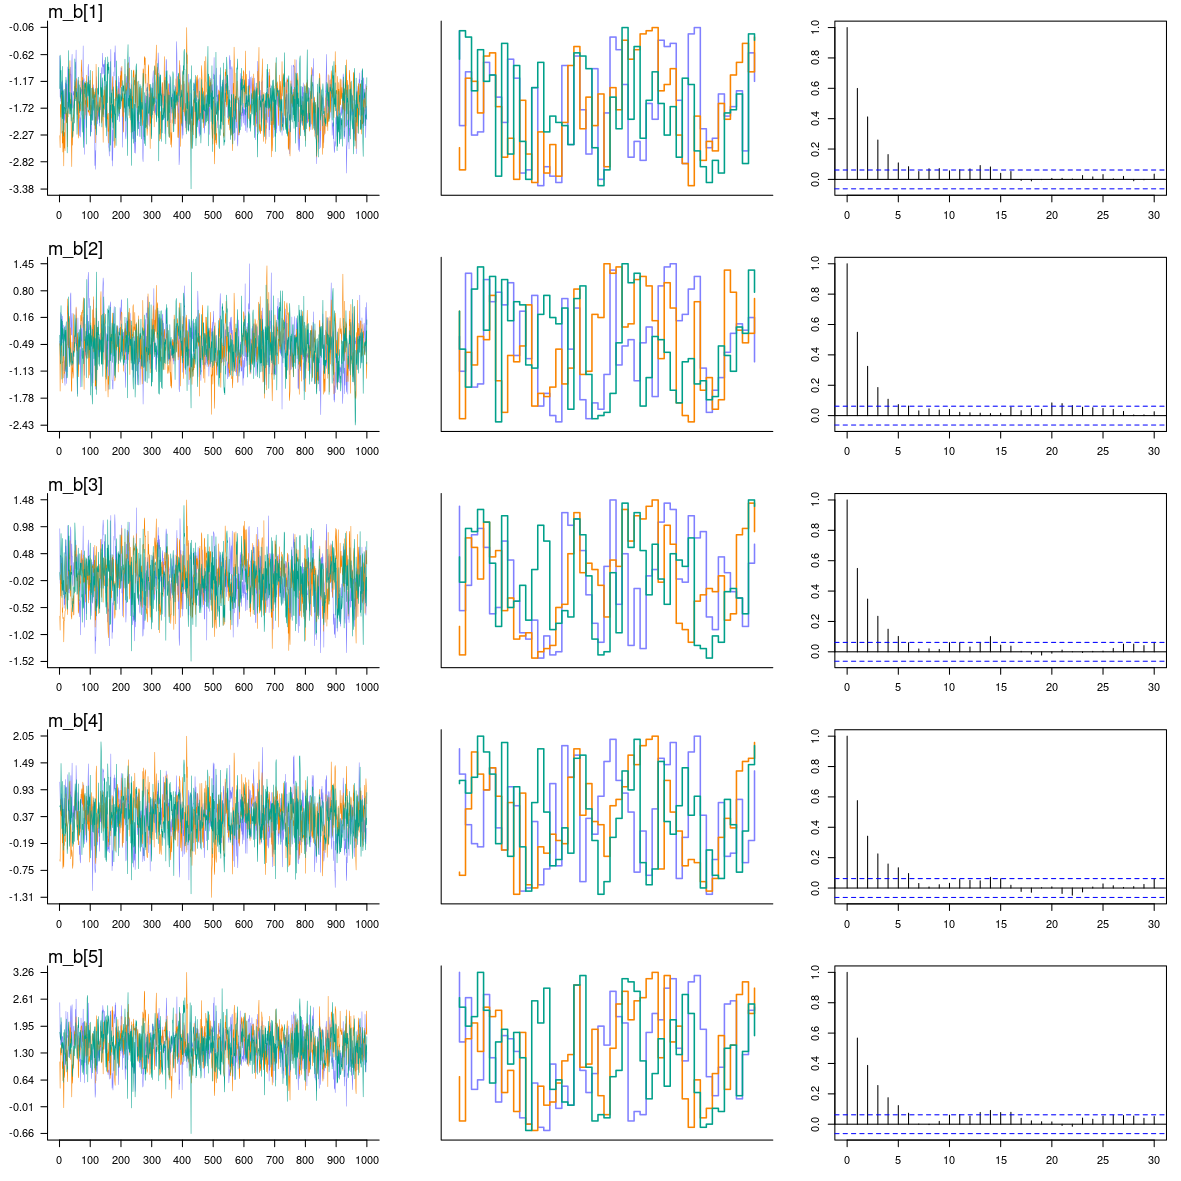
\includegraphics[width=1\linewidth]{FOLV_NC_J100_Ndata2_mb}
	%
	\caption[First-Order latent variable model (FOLV). Sample size $100$, replica number $2$. Non-centered parametrization. Mean difficulty per text. Trace, trank and auto-correlation plots.]%
	{First-Order latent variable model (FOLV). Sample size $100$, replica number $2$. Non-centered parametrization. Mean difficulty per text: (Left) trace plot, (Middle) trank plot, (Right) auto-correlation plot.}
	\label{fig:FOLV_NC_chains1}
\end{figure}
%
\begin{figure}[h]
	\centering
	\begin{subfigure}
		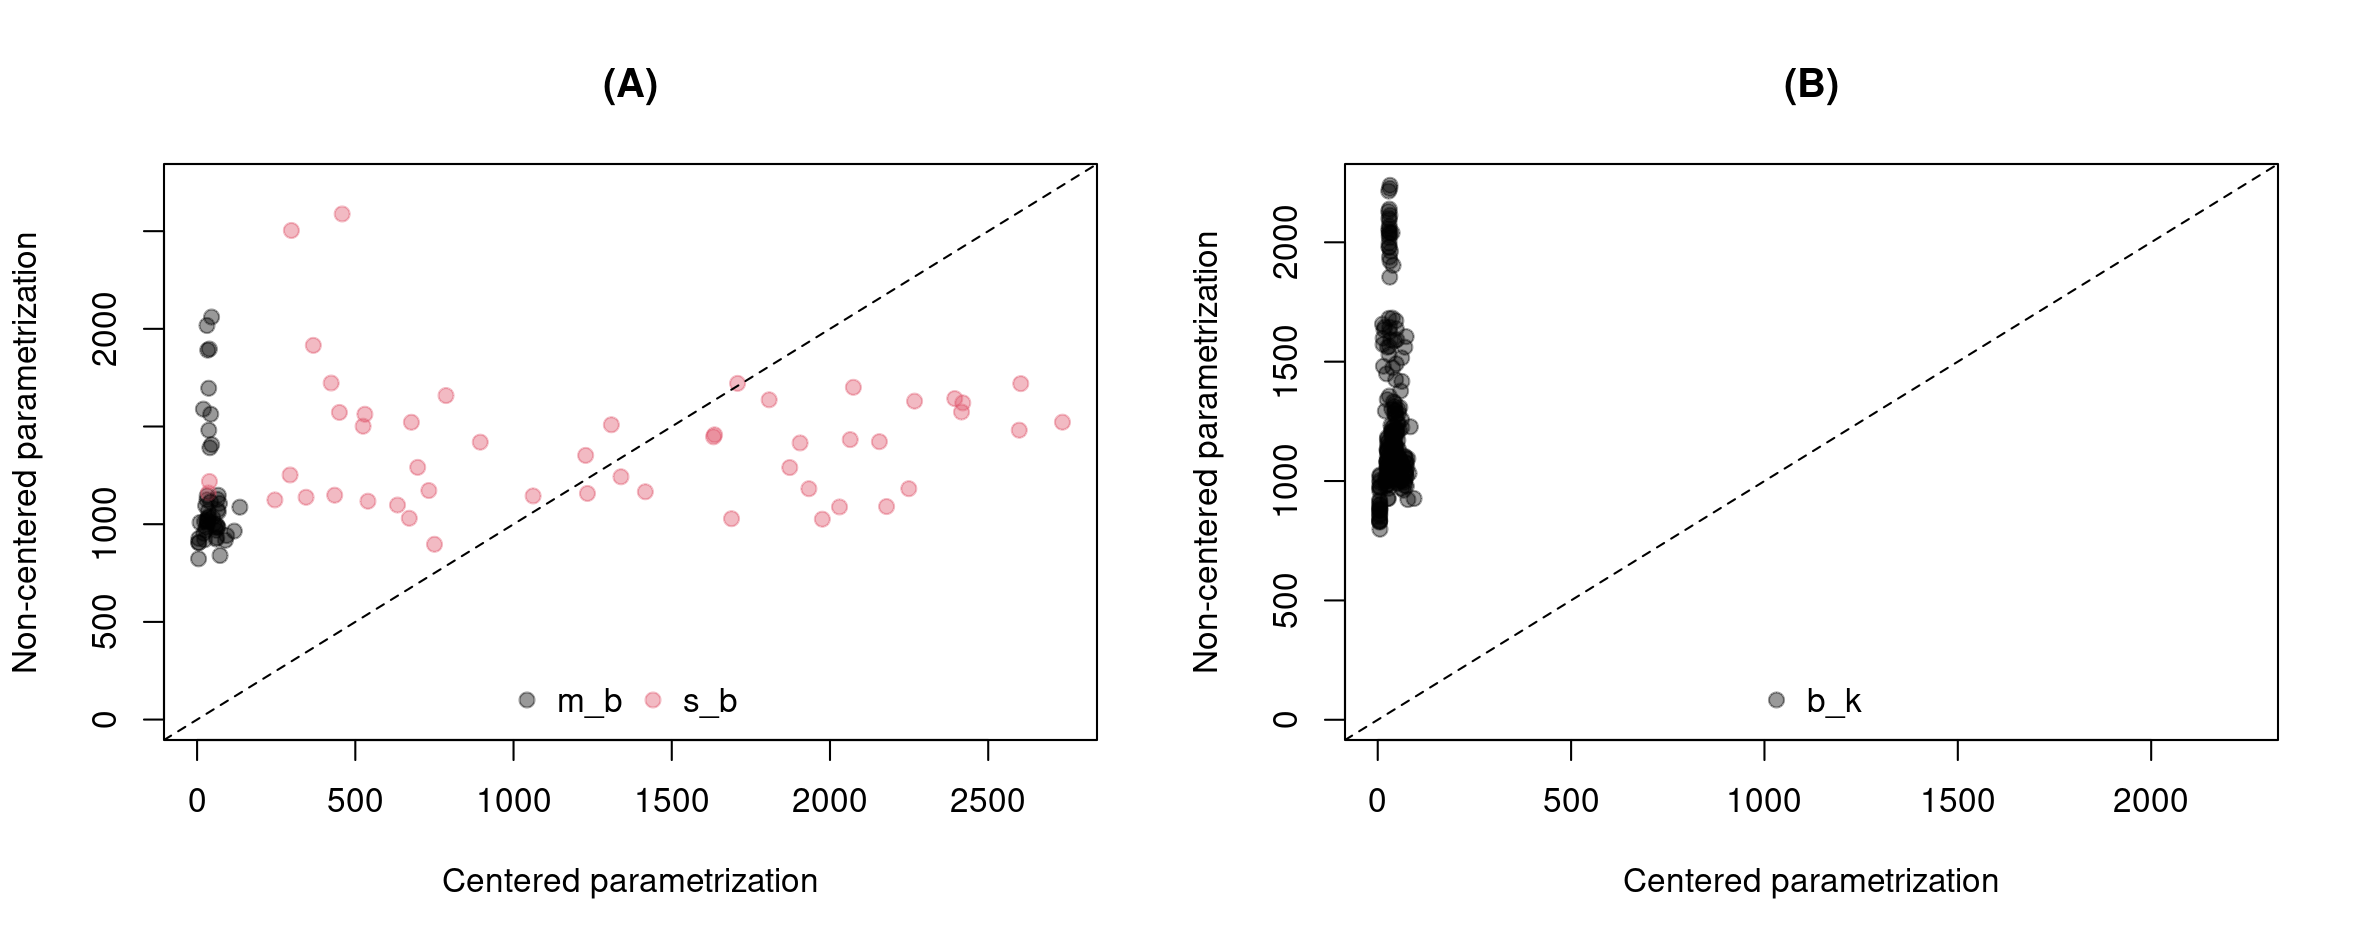
\includegraphics[width=1\linewidth]{FOLV_100_neff1}
	\end{subfigure}
	%
	\begin{subfigure}
		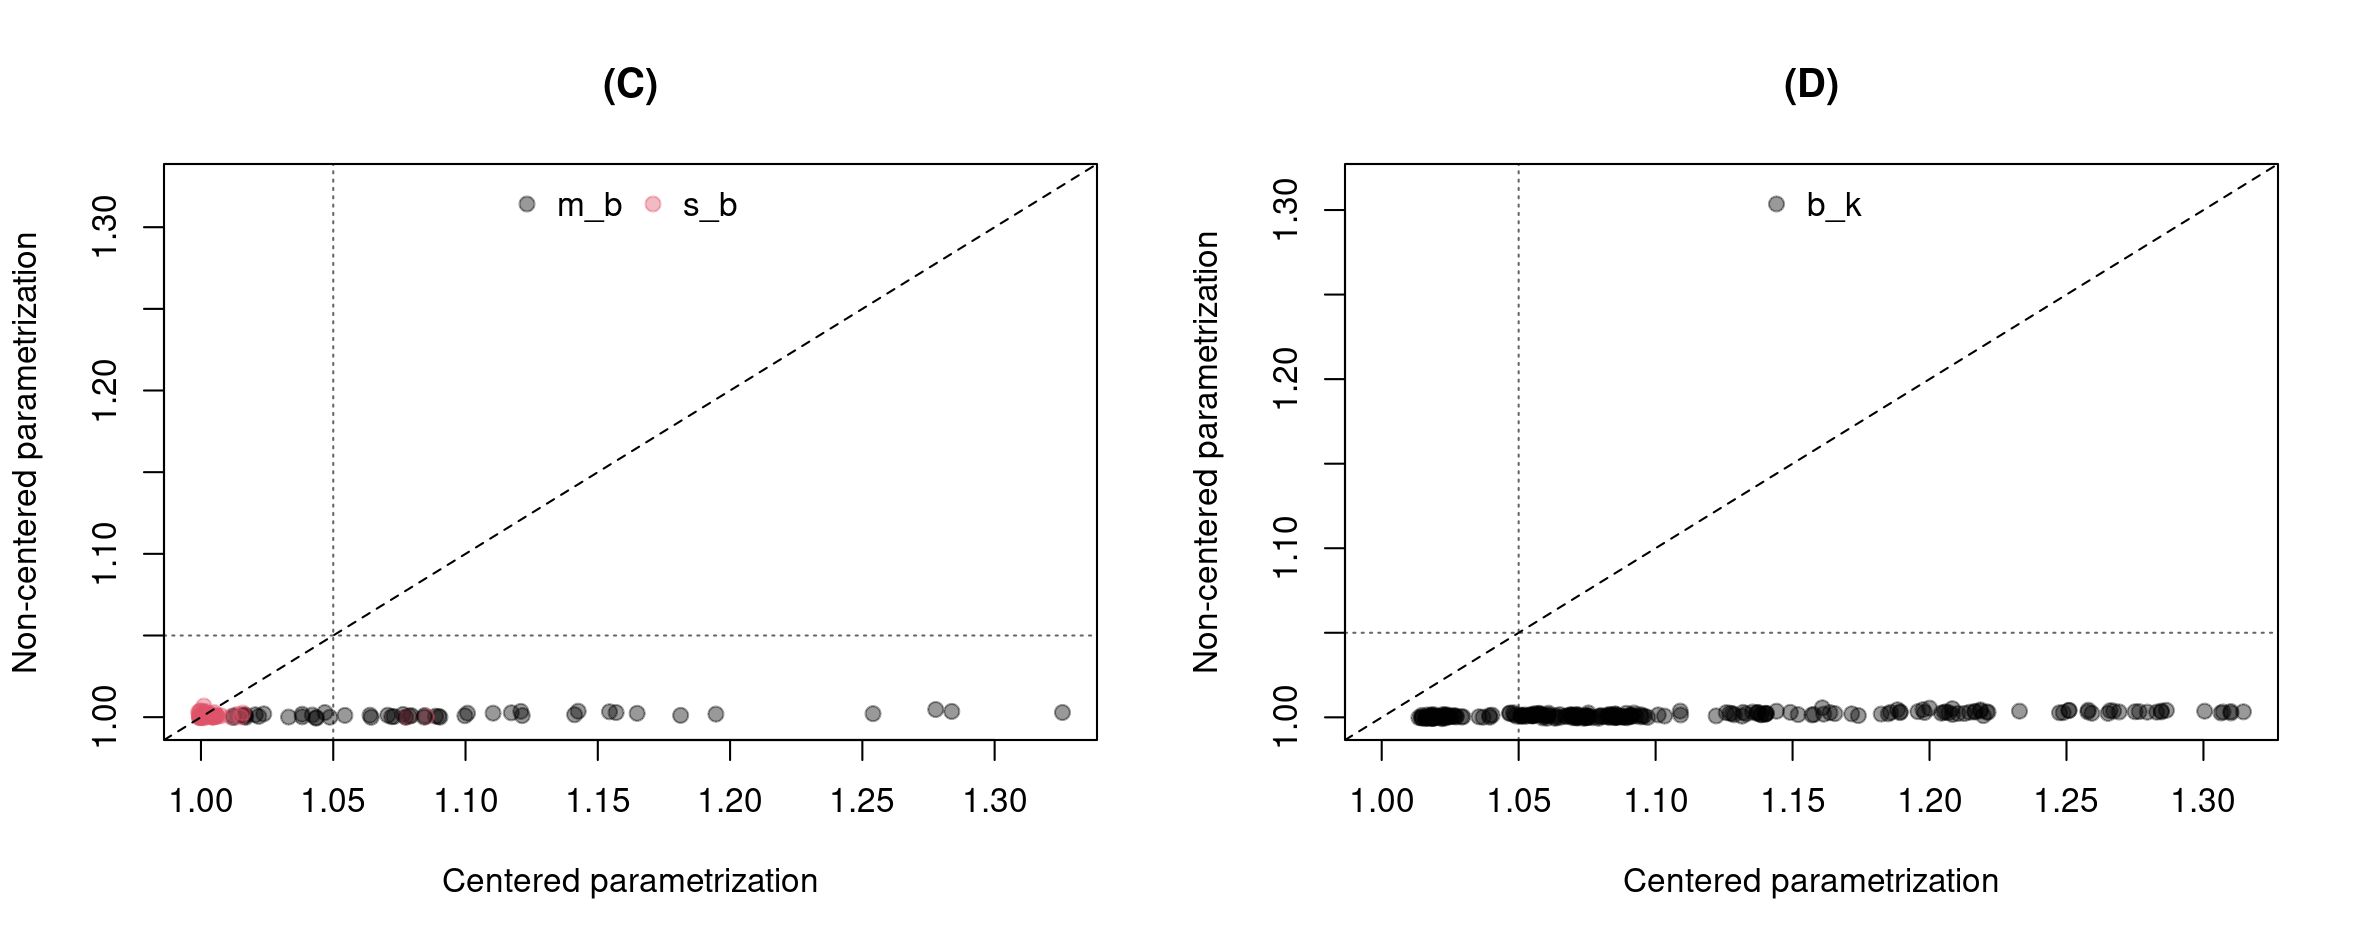
\includegraphics[width=1\linewidth]{FOLV_100_Rhat1}
	\end{subfigure}
	%
	\caption[First-order latent variable model (FOLV). Sample size $100$, all replicas. CP and NCP comparison plot.]%
	{First-order latent variable model (FOLV). Sample size $100$, all replicas. CP and NCP comparison plot. (A) \texttt{n\_eff} for texts' mean difficulty and standard deviation of difficulty. (B) \texttt{n\_eff} for items's difficulties. (C) \texttt{Rhat} for texts' mean difficulty and standard deviation of difficulty. (D) \texttt{Rhat} for items's difficulties. Diagonal discontinuous line describes equality between CP and NCP. Vertical and horizontal discontinuous lines is set at \texttt{Rhat}$=1.05$. }
	\label{fig:FOLV_stat1}
\end{figure}

So far we have only assessed specific replicas of the FOLV model, with a simulated sample size of $100$, as the previous paragraphs and title of the figures have indicated. However, after the inspection of the trace, trank, ACF and comparison plots\footnote{To inspect the remaining trace, trank, ACF, and comparison plots follow the github accompanying page detailed in Appendix \ref{sub_sect:chain_performance}.}, we notice the preceding patterns of stationarity, convergence and mixing extends to all replicas and simulated sample sizes in the FOLV model. Furthermore, the aforementioned patterns were also observed in the similar parameter set of the SOLV model. 

Additionally, for the remaining parameters in the SOLV, i.e. the loadings and reading comprehension higher-order latent variables, we continue observing the recurrent pattern between CP and NCP, detailed in previous paragraphs. Figures \ref{fig:SOLV_CE_chains1} and \ref{fig:SOLV_NC_chains1} show the NCP loadings have chains that seem slightly more stationary, convergent, and well mixed than its CP counterpart. This is further confirmed by panels (B) and (D) of figure \ref{fig:SOLV_stat1}. In a similar fashion, figures \ref{fig:SOLV_CE_chains3} and \ref{fig:SOLV_NC_chains3} show the higher-order latent variable is significantly more ergodic under the NCP than the CP, and figure \ref{fig:SOLV_stat2} confirms the hypothesis, by showing it has largely better effective sample sizes, with \texttt{Rhat} values always close to one.

Finally, panel (A) of figure \ref{fig:SOLV_stat3} show the pattern of ergodicity for the regression parameters is slightly improved under the SOLV\footnote{For the trace, trank and ACF plots refer to the corresponding accompanying page detailed in Appendix \ref{sub_sect:chain_performance}.}, i.e. the chains have larger effective sample sizes under the NCP versus the CP, indicating less correlation among the iterations, and therefore, better mixing. The result appear to be sensible, if we consider that the SOLV model was the data generating model.

Ultimately, the patterns for this set of parameters is also consistent across replicas and simulated sample sizes. Consequently, all of the above just show the NCP largely improved the performance of the MCMC chains under our implementation, for all models and almost all of the parameters. It is important to point out, the result did not extend to the sub-dimensions' correlation parameters, where no large difference was observed between the CP and NCP. On this matter, the issue was not related to a lack of identification of said parameters, as we were careful of ensuring this requirement.

\subsection{Recovery capacity}

\subsection{Retrodictive accuracy}

\subsection{Time}

\begin{table}[H]
	\centering
	\begin{tabular}{rlrrrr}
		\hline
		\multicolumn{3}{c}{ }& \multicolumn{3}{c}{ Time } \\ 
		\cmidrule(rl){4-6} 
		& Parametrization & Sample & mean & min & max \\ 
		\hline\hline
		1 & CP & 100 & 288.23 & 113.26 & 453.67 \\ 
		2 & CP & 250 & 470.85 & 335.86 & 994.39 \\ 
		3 & CP & 500 & 1149.25 & 1032.27 & 1351.92 \\ 
		4 & NCP & 100 & 116.49 & 104.35 & 133.99 \\ 
		5 & NCP & 250 & 430.86 & 406.58 & 503.91 \\ 
		6 & NCP & 500 & 1342.93 & 1207.00 & 1717.22 \\
		\hline
	\end{tabular}
	\caption[FOLV running time statistics.]%
	{FOLV running time statistics.} 
	\label{tab:FOLV_time}
\end{table}

\begin{table}[H]
	\centering
	\begin{tabular}{rlrrrr}
		\hline
		\multicolumn{3}{c}{ }& \multicolumn{3}{c}{ Time } \\ 
		\cmidrule(rl){4-6} 
		& Parametrization & Sample & mean & min & max \\ 
		\hline\hline
		1 & CP & 100 & 242.30 & 83.54 & 513.22 \\ 
		2 & CP & 250 & 428.00 & 313.32 & 689.50 \\ 
		3 & CP & 500 & 968.54 & 867.03 & 1183.53 \\ 
		4 & NCP & 100 & 112.33 & 97.27 & 136.72 \\ 
		5 & NCP & 250 & 355.01 & 311.75 & 407.40 \\ 
		6 & NCP & 500 & 994.65 & 802.05 & 1095.33 \\ 
		\hline
	\end{tabular}
	\caption[SOLV running time statistics.]%
	{SOLV running time statistics.} 
	\label{tab:SOLV_time}
\end{table}
